%%%%%%%%%%%%%%%%%%%%%%%%%%%%%%%%%%%%%%%%%%%%%%%%%%%%%%%%%%%%%%%%%%%%%%%%%%%%%%%
% Chapter 3: Título del capítulo 3
%%%%%%%%%%%%%%%%%%%%%%%%%%%%%%%%%%%%%%%%%%%%%%%%%%%%%%%%%%%%%%%%%%%%%%%%%%%%%%%

\section{Tecnologías}
\label{3:sec1}

\subsection{Tecnologías populares}
\label{3:1:1}
{\bf Django - Python}
Django es un framework para aplicaciones web gratuito y open source, escrito en Python. Un conjunto de componentes que te ayudan a desarrollar sitios web más fácil y rápidamente siguiendo el patrón Modelo Vista Controlador.

{\bf Ruby on Rails - Ruby}
Ruby on Rails, también conocido como RoR o Rails, es un framework de aplicaciones web de código abierto escrito en el lenguaje de programación Ruby, siguiendo el patrón Modelo Vista Controlador (MVC).

{\bf Express.js - Javascript}
Espress.js  es un framework de desarrollo de aplicaciones web minimalista y flexible para Node.js. Está inspirado en Sinatra, además es robusto, rápido, flexible y muy simple, además, es compatible con el patrón Modelo Vista Controlador.

Aquí tenemos una pequeña comparación de la popularidad que han tenido estas tecnologías en el último año.

\begin{figure}[!th]
\begin{center}
\includegraphics[scale=0.6]{images/comparativa}
\caption{Comparativa de Tecnologias usadas}
\label{fig:Comparativa de Tecnologias usadas}
\end{center}
\end{figure}


%++++++++++++++++++++++++++++++++++++++++++++++++++++++++++++++++++++++++++++++

\subsection{Tecnologías Escogidas}
\label{3:1:2}

Finalmente se escogió Express.js, Node.js y Javascript como tecnologías principales a usar en este proyecto por las siguientes razones:

En primer lugar, el uso de Node.js como tecnología de servidor aporta una gran ventaja ya que Javascript se usa en ambos lados, en el backend y en el frontend, reduciendo complejidad y tiempo de desarrollo ya que Express es bastante fácil de aprender y usar. Además, JavaScript es el lenguaje de programación más popular en el desarrollo web.

Además de eso, la comunidad de Node.js está en constante crecimiento: la cantidad de preguntas de StackOverflow aumenta constantemente, por lo que la base de conocimiento para la tecnología es amplia. También hay que destacar el hecho de que Node.js sea de código abierto y gratuito. 

Finalmente, Node nos ofrece NPM, un gestor de paquetes que dispone de una gran cantidad de paquetes que crece rápidamente y aporta una forma sencilla de gestionar los paquetes que necesitemos en nuestro proyecto.

{\bf NPM}

NPM es un administrador de paquetes para Node.js con cientos de miles de paquetes. Aunque crea parte de la estructura del directorio del proyecto, este no es el objetivo principal.

El objetivo principal, es la automatización de dependencias y gestión de paquetes de cada proyecto. Esto significa que puede especificar todas las dependencias de su proyecto dentro del fichero package.json usando el comando npm i -s nombrepaquete, de forma que cada vez que un usuario clone el proyecto en su máquina simplemente tenga ejecutar npm install e inmediatamente se descargan e instalan todas las dependencias necesarias para el funcionamiento del proyecto en el directorio node modules/. Además, también sirve para especificar en qué versión está su proyecto.

También es posible descargar manualmente los paquetes, copiarlo en el directorio nodemodules/ y usarlo de esa manera. Sin embargo, a medida que crezca el proyecto y la lista de dependencias, llevará mucho tiempo instalar los paquetes necesarios y será una tarea engorrosa. También hace que colaborar y compartir tu proyecto sea mucho más difícil

{\bf Express.js}

Express es un framework ‘’minimalista’’ que permite crear una infraestructura web simple sobre Node.js. Express permite crear una API REST, un tipo de arquitectura de desarrollo web que se apoya totalmente en el estándar HTTP:

\begin{itemize}
  \item GET: Para consultar y leer recursos
  \item POST: Para crear recursos
  \item PUT: Para editar recursos
  \item DELETE: Para eliminar recursos
  \item PATCH: Para editar partes concretas de un recurso
\end{itemize}

Express también permite crear una aplicación web siguiendo el patrón de diseño Modelo Vista Controlador, que separa los datos y la lógica de de una aplicación de su representación.

{\bf Github API}

Para poder usar Github como estructura necesitaremos hacer uso de su Github REST API v3. 
La API nos permitirá acceder a los servicios que ofrece Github de forma externa, es decir, podremos crear repositorios, usar organizaciones como clases y manejar otros servicios, como consulta de información sobre el usuario.
Para poder acceder a la clave de cada usuario, debemos usar un Token generado por Github, es decir, una cadena que nos permitirá  identificarnos para realizar transacciones usando la API, en este caso, el token será generado usando las aplicaciones OAuth que nos ofrece Github para que el usuario haga login con su cuenta de usuario de github, sin necesidad de poner su usuario y contraseña de Github en la plataforma Codelab.
La Github REST API v3 tiene además varias librerías de terceros y tres librerías oficiales escritas en Ruby, Javascript y .Net.

{\bf MongoDB}

MongoDB es un sistema gestor de base de datos NoSQL, es decir, MongoDB es un sistema de bases de datos no relacional, en lugar de almacenar los datos en tablas, se almacenan colecciones o documentos, que está formado por objetos, y estos a su vez por claves y cada clave tiene un valor asociado. Es decir, sería algo parecido a un documento JSON, aunque en MongoDB usan una distribución llamada BSON.

\begin{figure}[!th]
\begin{center}
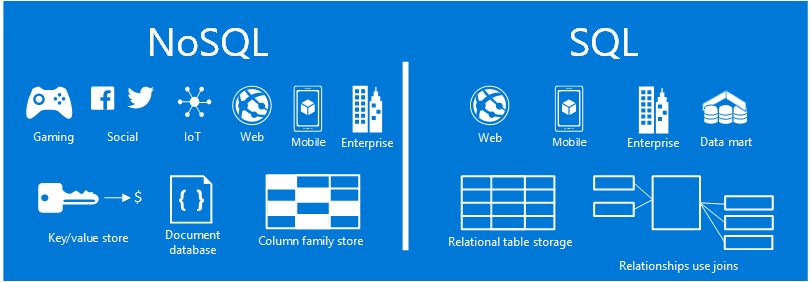
\includegraphics[scale=0.5]{images/nosql}
\caption{NoSQL vs SQL}
\label{fig:NoSQL vs SQL}
\end{center}
\end{figure}

{\bf Mongoose}

Mongoose es un una herramienta para el diseño de objetos de MongoDB. 
Mongoose provee una serie de métodos y funciones para manejar la base de datos en MongoDB.

{\bf Motor de vistas}

Como motor de vistas para el proyecto se ha elegido Pug, antes conocido como Jade, un motor de vistas implementado en Javascript para su uso en NodeJS y que dispone de una fácil integración con Express.JS. 

{\bf Automatización de tareas}

Para la automatización de tareas como generar el fichero de variables de entorno o poner en marcha un servidor nodemon se ha usado Gulp, una herramienta que permite automatizar tareas en Node.js, es simple y bastante fácil de usar.

{\bf Framework de CSS}

Como framework para los estilos de CSS se ha usado Materialize CSS, basado en material design. Ofrece varias opciones a la hora de diseñar la plataforma, permitiendo un diseño más minimalista o un diseño más cargado y vistoso.

%++++++++++++++++++++++++++++++++++++++++++++++++++++++++++++++++++++++++++++++
\section{Github API}
\label{3:sec2}

Para poder usar Github como estructura para la creación de aulas y tareas de código usaremos la Github REST API V3.
La API permite acceder a las funcionalidades de Github

%++++++++++++++++++++++++++++++++++++++++++++++++++++++++++++++++++++++++++++++
\section{Tercera sección de este capítulo}
\label{:sec3}
